\documentclass{beamer}
\usetheme{Warsaw}

\usepackage[utf8]{inputenc}
\usepackage{fancybox}
\usepackage{multimedia} 
\usepackage{subfig}
\usepackage{amsmath}
\usepackage{hyperref}
\usepackage[all]{xy}
\usepackage{algorithm}
%\usepackage{arevmath}     % For math symbols
\usepackage[noend]{algpseudocode}

\begin{document}


\title[Angewandte Mathematik] % (optional, only for long titles)
{Angewandte Mathematik
\\
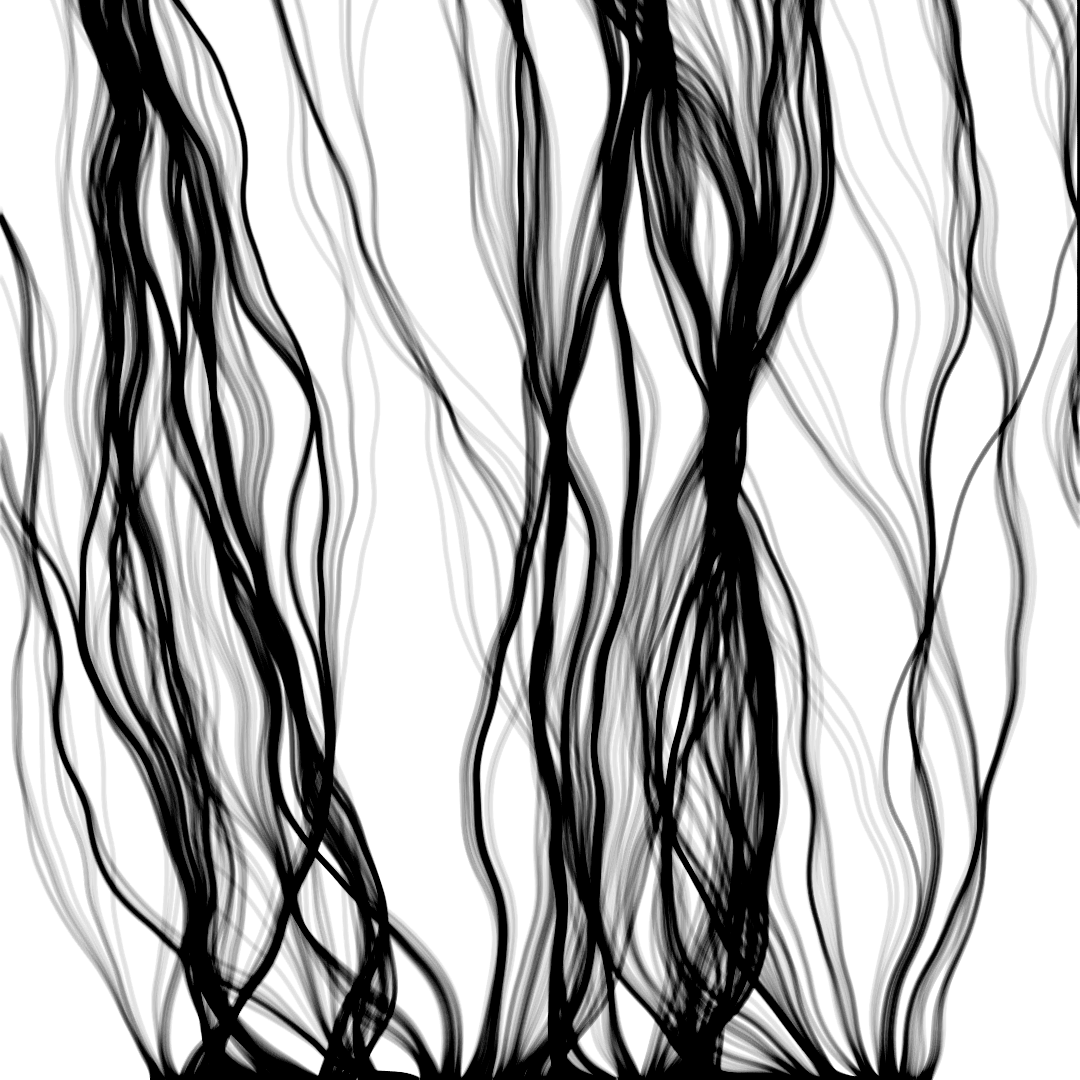
\includegraphics[scale=0.15]{images/cover}
}
\subtitle{}
\author[Dr. Johannes Riesterer] % (optional, for multiple authors)
{Dr.  rer. nat. Johannes Riesterer}

\date[KPT 2004] % (optional)
{}

\subject{Angewandte Mathematik}



\frame{\titlepage}



\begin{frame}
    \frametitle{Angewandte Mathematik}
\framesubtitle{Dynamische Systeme Systeme}
\begin{block}{Motivation}
Gegeben ist ein zeitabhängiges System $t \mapsto x(t)$. Möchten verstehen, wie sich $x(t)$ über die Zeit entwickelt. Zu festen Zeitpunkten $t_0, \cdots t_n $ lässt sich $x(t_i)$ messen und damit $x'(t_i) \cong \frac{x(x(t_i) - x(t_{i-1}))}{t_i - t_{i-1}}$ näherungsweise bestimmen. Im allgemeinen ist $x'(t) = f(x(t), t)$. 
\end{block}
 \end{frame}

\begin{frame}
    \frametitle{Angewandte Mathematik}
\framesubtitle{Dynamische Systeme Systeme}
\begin{block}{Beispiel}
$(1) \;x'(t) = \mu e^{x}$.  Dann ist $x(t)= c e^{\mu t}$ für alle $c \in \mathbb{R}$ eine Lösung. Ist $x(0) = x_0$, so ist   $x(t)= x_0 e^{\mu t}$ eine Lösung von (1) mit $x(0) = x_0$. 
\end{block}
 \end{frame}

\begin{frame}
    \frametitle{Angewandte Mathematik}
\framesubtitle{Dynamische Systeme Systeme}
\begin{block}{System von Differentialgleichungen}
Ein System von Differentialgleichungen $1$-ter Ordnung ist ein System von Gleichungen
\begin{align*}
\begin{matrix} x_1'(t) = f_1(t, x_1, \cdots, x_n ) \\  \\ x_2'(t) = f_1(t, x_1, \cdots, x_n ) \\  \vdots \\  x_n'(t) = f_1(t, x_1, \cdots, x_n )\end{matrix}
\end{align*}
Werden zusätzlich die Anfanfsbedingungen $x_1(t_0)= x_0^1; \dots x_n(t_0) = x_0^n$ vorgegebenen, so spricht man von einem Anfangswertproblem.
Eine Lösung ist eine Funktion $x : I \subset \mathbb{R} \to \mathbb{R}^n$, deren Koordinatenfunktionen diese Bedingungen erfüllt.
\end{block}
 \end{frame}

\begin{frame}
    \frametitle{Angewandte Mathematik}
\framesubtitle{Dynamische Systeme Systeme}
\begin{block}{System von Differentialgleichungen}

Ein Anfangswertproblem $n$-ter Ordnung
 $$ x^{(n)}(t) = f(t, x^{(n)}, x^{(n-1)} , \cdots , x', x) $$ mit  $x(t_0) = x_0 ; x'(t_0) = x_1; \cdots ; x^{n-1}(t_{0})= x_{n-1}  $ ist äquivalent zu dem System von   Differentialgleichungen $1$-ter Ordnung
\begin{align*}
\begin{matrix} x_1'(t) = x_2(t) \\  \\ x_2'(t) = x_3(t) \\  \vdots  \\ x_n'(t) = f(t, x_1, \cdots, x_n )\end{matrix}
\end{align*}
mit den Anfangswertbedingungen  $x_1(t_0) = x_0 ; x_2(t_1) = x_1; \cdots ; x_{n-1}(t_{0})= x_{n-1} $.
\end{block}
 \end{frame}


\begin{frame}
    \frametitle{Angewandte Mathematik}
\framesubtitle{Dynamische Systeme Systeme}
\begin{block}{System von Differentialgleichungen}
Ein Vektorfeld ist eine Abbildung $$v : \Omega \subset \mathbb{R}^n \to \mathbb{R}^n \; ,$$ die jedem Punkt $x  \in \Omega$ einen Vektor $v(x) \in \mathbb{R}^n$ zuordnet.
\end{block}
\begin{figure}[H]
      \centering
    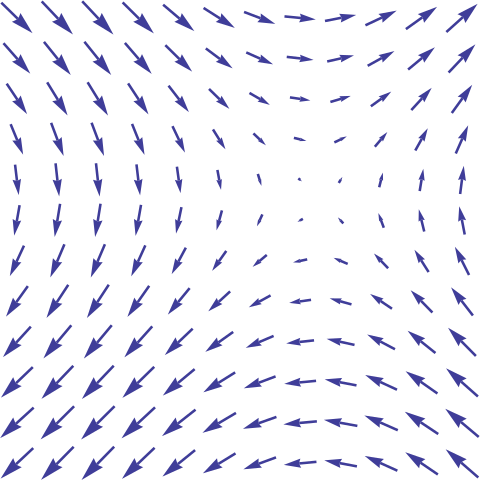
\includegraphics[width=0.3\textwidth]{images/480px-VectorField.png}
\caption{Quelle: Wikipedia:https://en.wikipedia.org/wiki/Vector\_field\#/media/File:VectorField.svg}
\end{figure}

 \end{frame}

\begin{frame}
    \frametitle{Angewandte Mathematik}
\framesubtitle{Dynamische Systeme Systeme}
\begin{block}{System von Differentialgleichungen}
Eine Weg $\varphi : I \subset \mathbb{R} \to \mathbb{R}^n$ heißt Integralkurve in dem Vektorfeld $v : \Omega \subset \mathbb{R}^n \to \mathbb{R}^n$, falls 
$$\varphi' (t) = v(\varphi(t))$$ gilt für alle $t \in  I$.
\end{block}
\begin{figure}[H]
      \centering
    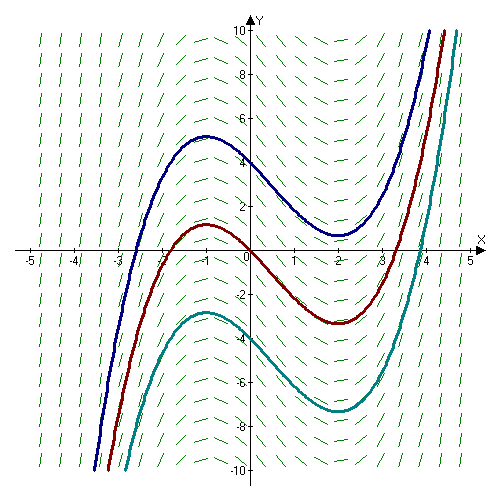
\includegraphics[width=0.3\textwidth]{images/Slope_Field.png}
\caption{Quelle: Wikipedia:https://en.wikipedia.org/wiki/Integral\_curve\#/media/File:Slope\_Field.png}
\end{figure}

 \end{frame}


\begin{frame}
    \frametitle{Angewandte Mathematik}
\framesubtitle{Dynamische Systeme Systeme}
\begin{block}{System von Differentialgleichungen}
Ein dynamisches System ist eine  Abbildung $F : U \subset \mathbb{R} \times \mathbb{R}^n \to \mathbb{R}^n$, die jedem Punkt $(t,x)  \in U$ einen Vektor $F(t,x) \in \mathbb{R}^n$ zuordnet. Eine Integralkurve oder Lösung für $F$ ist eine Weg $\varphi : I \to \mathbb{R}^n$ mit 
$$\varphi'(t) = F(t, \varphi(t)) $$
für alles $t \in I$.
\end{block}
 \end{frame}


\begin{frame}
    \frametitle{Angewandte Mathematik}
\framesubtitle{Dynamische Systeme Systeme}
\begin{block}{System von Differentialgleichungen}

Für eine  vektorwertige Funktion  $f : I   \to \mathbb{R}^n; f(t) : = \begin{pmatrix} f_1(t)  \\ \vdots \\ f_n(t) \end{pmatrix}$ definieren wir das Integral komponentenweise durch
$$\int_{a}^{b}  f(t) dt := \begin{pmatrix} \int_{a}^{b}  f_1(t) dt  \\ \vdots \\ \int_{a}^{b}  f_n(t) dt \end{pmatrix} \; .$$
\end{block}
 \end{frame}

\begin{frame}
    \frametitle{Angewandte Mathematik}
\framesubtitle{Dynamische Systeme Systeme}
\begin{block}{System von Differentialgleichungen}
Ein Weg $\varphi : I \subset \mathbb{R} \to \mathbb{R}^n$ ist genau dann Lösung des AWP $\varphi'(t) = F(t , \varphi)$ mit $ \varphi(t_0)= x_0$, wenn
$$ \varphi(t) =  x_0 + \int_{t_0}^{t} F(t, \varphi) dt$$
gilt.
\end{block}
\begin{block}{Beweis}
Folgt direkt durch komponentenweise Anwendung des Hauptsatzes der Integral- und Differentialrechnung.
\end{block}
 \end{frame}


\begin{frame}
    \frametitle{Angewandte Mathematik}
\framesubtitle{Dynamische Systeme Systeme}
\begin{block}{Lipschitz-Stetig}
Eine  Abbildung $F : U \subset \mathbb{R} \times \mathbb{R}^n \to \mathbb{R}^n$ heißt Lipschitz-Stetig,
falls es eine Konstante $L \geq 0$ gibt  mit
$$ || F(t,x) - F(t,x') ||  \leq L || x -x' ||  $$
für alle $(t,x)$ und $(t,x')$ in $U$.
\end{block}

 \end{frame}


\begin{frame}
    \frametitle{Angewandte Mathematik}
\framesubtitle{Dynamische Systeme Systeme}
\begin{block}{Metrischer Raum}
Ein metrischer Raum $(X,d)$ ist eine Menge $X$ zusammen mit einer Abbildung $d : X \times X \to X$ die linear ist in beiden Argumenten und die Dreiecksungleichung $d(x,y) \leq d(x,z) + d(z,y)$ erfüllt.  
\end{block}
\begin{block}{Beispiel}
$d(x,y) : = || y- x  ||$  wobei $||  \cdot ||$  eine Norm ist. 
\end{block}

\begin{block}{Beispiel}
Das für uns später relevante Beispiel ist der Funktionenraum mit der Maximumsnorm $|| \varphi || := \max_t$.
\end{block}
 \end{frame}


\begin{frame}
    \frametitle{Angewandte Mathematik}
\framesubtitle{Dynamische Systeme Systeme}
\begin{block}{Banachscher Fixpunktsatz}
Es sei $(X,d)$ ein vollständiger metrischer Raum und $P: X \to X$ eine Abbildung mit $$d(P(x), P(x)) < \lambda d(x,y)$$ und $\lambda < 1$. Dann besitzt $P$ genau einen Fixpunkt $x^* \in X$ mit $P(x^*) = x^*$.

\end{block}

 \end{frame}

\begin{frame}
    \frametitle{Angewandte Mathematik}
\framesubtitle{Dynamische Systeme Systeme}
\begin{figure}[H]
      \centering
    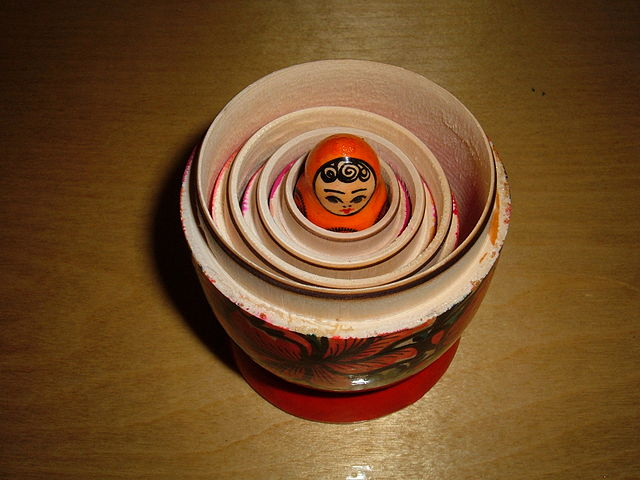
\includegraphics[width=0.7\textwidth]{images/640px-Floral_matryoshka_set_2_smallest_doll_nested.JPG}
\caption{Quelle: Wikipedia}
\end{figure}

 \end{frame}


\begin{frame}
    \frametitle{Angewandte Mathematik}
\framesubtitle{Beweis}
Wähle beliebiges $x_0 \in X$. Durch wiederholtes Abbilden erhalten wir die Folge  $x_n:= P(x_{n-1})$. Für diese Gilt nach Voraussetzung an $P$
\begin{align*}
d(x_{n+1} , x_{n}) < \lambda d(x_{n} , x_{n-1})   < \lambda^n d(x_{1} , x_{0})  \; .
\end{align*}
Mit wiederholtem Anwenden der Dreiecksungleichung gilt 
\begin{align*}
d(x_{n + m} , x_{ m}) \leq d(x_{n+1} , x_{n})  +  d(x_{n +2} , x_{n +1}) +   \cdots   +  d(x_{n + m } , x_{n +m -1}) \; .
\end{align*}
Da $\lambda < 1$ folgt $  \lim_{n \to \infty} d(x_{n + m} , x_{ m})   \leq  \lim_{n \to \infty} \frac{\lambda^n}{1 - \lambda} d(x_{1} , d_{0}) = 0$ und damit ist $x_n$ eine Cauchyfolge.  Da $(X,d)$ vollständig ist, konvergiert die Folge in $X$ gegen einen Grenzwert $x^*$. Für diesen gilt $P(x^*) =  P (  \lim_{n \to \infty}  x^*) =  \lim_{n \to \infty} P(x_n)  =  \lim_{n \to \infty} x_{n+1} = x^*$ und damit ist $x^*$ ein Fixpunkt von $P$.

 \end{frame}

\begin{frame}
    \frametitle{Angewandte Mathematik}
\framesubtitle{Dynamische Systeme Systeme}
\begin{block}{Lokaler Existenzsatz von Picard-Lindelöf}
Das dynamisches System  $$F : U \subset \mathbb{R} \times \mathbb{R}^n \to \mathbb{R}^n$$ sei lokal Lipschitz-Stetig. 
Dann gibt es zu jedem Punkt $(t_0, x_0) \in U$ ein Intervall $I_\delta (t_0) := (t_0 - \delta, t_0 + \delta) \subset \mathbb{R}$ auf dem das AWP 
$$ x' = F(t,x), \; \; x(t_0) = x_0$$
\end{block}

 \end{frame}

\begin{frame}
    \frametitle{Angewandte Mathematik}
\framesubtitle{Beweis}

 \end{frame}



\begin{frame}
    \frametitle{Angewandte Mathematik}
\framesubtitle{Dynamische Systeme Systeme}
\begin{block}{Lineare (gewöhnliche) Differentialgleichung.}
Eine Differentialgleichung der Form
$$ x' (t): = A(t) x(t) + b(t)$$
mit $A: I \subset \mathbb{R} \to \mathbb{R}^{n \times n}$ und $b: I \subset \mathbb{R} \to \mathbb{R}^{n}$ heißt lineare (gewöhnliche) Differentialgleichung.
\end{block}

 \end{frame}


\begin{frame}
    \frametitle{Angewandte Mathematik}
\framesubtitle{Dynamische Systeme Systeme}
\begin{block}{Existenz und Eindeutigkeit]}
Ist $x' (t): = A(t) x(t) + b(t)$ eine lineare Differentialgleichung und $A$ und $b$ stetig, so besitzt das AWP 
$$ x' (t): = A(t) x(t) + b(t) ; \; \; x(t_0) = x_0 $$
genau eine auf ganz $I$ definierte Lösung.
\end{block}
\begin{block}{Beweis}
$F(t,x):= A(t) x(t) + b(t)$ ist Lipschitz-Stetig mit Konstanten $L:= \max_{t \in J}|| A(t) ||$ für jedes kompakte Intervall $J \subset I$.
\end{block}
 \end{frame}


\begin{frame}
    \frametitle{Angewandte Mathematik}
\framesubtitle{Dynamische Systeme Systeme}
\begin{block}{Lineare (gewöhnliche) Differentialgleichung.}
\begin{itemize}
\item Die Menge $\mathcal{L}$ der auf $I$ definierten Lösungen der homogenen Gleichung $x'(t) = A(t)x(t)$ ist eine $n$-dimensionaler reeller Vektorraum.
\item $n$ Lösungen $\varphi_1, \cdots, \varphi_n : I \to \mathbb{R}^n$ bilden genau dann eine Basis für $\mathcal{L}$, wenn die Vektoren $\varphi_1(t), \cdots, \varphi_n(t)$ für ein $t \in I$ eine Basis des $\mathbb{R}^n$ bilden.
\end{itemize}
\end{block}

 \end{frame}


\begin{frame}
    \frametitle{Angewandte Mathematik}
\framesubtitle{Beweis}
Sind  $\varphi_1, \cdots, \varphi_n$ Lösungen der homogenen Gleichung, so auch $ c_1 \cdot \varphi_1 + \cdots + c_n \cdot \varphi_n$, da die Ableitung linear ist.
$\mathcal{L}$ ist somit ein Vektorraum. Definiere 
\begin{align*}
& \alpha_{t_0} : \mathcal{L} \to \mathbb{R}^n \\
& \alpha_{t_0} (\varphi) := \varphi(t_0) \; .
\end{align*} 
Aufgrund des Existenzsatzes und der linearität ist $ \alpha_{t_0}$ surjektiv und wegen der Eindeutigkeit der Lösung injektiv.
 \end{frame}


\begin{frame}
    \frametitle{Angewandte Mathematik}
\framesubtitle{Dynamische Systeme Systeme}
\begin{block}{Lineare (gewöhnliche) Differentialgleichung.}
Eine Basis  $\varphi_1, \cdots, \varphi_n$ des Lösungsraumes $\mathcal{L}$ der homogenen Gleichung $x'(t) = A(t)x(t)$ heißt Fundamentalsystem.
\end{block}

 \end{frame}

\begin{frame}
    \frametitle{Angewandte Mathematik}
\framesubtitle{Dynamische Systeme Systeme}
\begin{block}{Lineare (gewöhnliche) Differentialgleichung.}
Für eine Matrix $A \in \mathbb{R}^{n \times n}$ definiert man die Exponentialfunktion 
$$  e^{ A}  := \sum_{k= 0}^{\infty} \frac{1}{k!} A^k \; .$$
Es gilt  
$$  (e^{ tA})' = A e^{tA}  \; .$$
\end{block}

 \end{frame}

\begin{frame}
    \frametitle{Angewandte Mathematik}
\framesubtitle{Dynamische Systeme Systeme}
\begin{block}{Lineare (gewöhnliche) Differentialgleichung.}
Für eine Matrix $A$ lautet die Lösung des Anfangswertproblems $x'(t) = Ax(t)$ und $x(0) = x_0$
$$ x(t) = e^{tA} x_0 \;.$$ Ist $v_1, \cdots , v_n$ eine Basis des $\mathbb{R}^n$, so ist $e^{tA}v_1, \cdots , e^{tA}v_n$ ein Fundamentalsystem für $\mathcal{L}$. Damit bilden die Spalten von  $e^{tA}$ ein Fundamentalsystem.
\end{block}

\begin{block}{Beweis}
Es ist $x(0) = x_0$ und $x'(t)= A x(t)$. Der Rest folgt aus Satz  \ref{LHL}
\end{block}
 \end{frame}


\begin{frame}
    \frametitle{Angewandte Mathematik}
\framesubtitle{Dynamische Systeme Systeme}
\begin{block}{Lineare (gewöhnliche) Differentialgleichung.}
Sei $v$ eine Eigenvektor von $A$ zum Eigenwert $\lambda$. Dann löst 
$$ \varphi_v(t) := e^{t \lambda} v$$ das AWP $x' = Ax$ mit $x(0) = v$.

\end{block}
\begin{block}{Beweis}
$\varphi_v'(t) =  \lambda  e^{t \lambda}  v =  e^{t\lambda}  \lambda v =  e^{t\lambda}  A v  = A e^{t\lambda}   v  = A  \varphi_v(t)$.

\end{block}
 \end{frame}

\begin{frame}
    \frametitle{Angewandte Mathematik}
\framesubtitle{Dynamische Systeme Systeme}
\begin{block}{Lineare (gewöhnliche) Differentialgleichung.}
Hat eine Matrix $A$ $n$ Eigenvektoren $v_1, \cdots , v_n$ zu den Eigenwerten $\lambda_1, \cdots  \lambda_n$, 
so bilden die Lösungen $ \varphi_{v_1}, \cdots  \varphi_{v_n}$ ein Fundamentalsystem.
\end{block}
\begin{block}{Beweis}
Eigenvektoren sind linear unabhängig.
\end{block}
 \end{frame}


\begin{frame}
    \frametitle{Angewandte Mathematik}
\framesubtitle{Dynamische Systeme Systeme}
\begin{block}{Hauptvektoren.}
Ein Vektor $v$ heißt Hauptvektor zum Eigenwert $\lambda$, falls es eine Zahl $s>0$ gibt mit 
$$ (A - \lambda E)^s v = 0$$
Die kleinste Zahl $s$, für die dies gilt heißt Stufe.
\end{block}

 \end{frame}


\begin{frame}
    \frametitle{Angewandte Mathematik}
\framesubtitle{Dynamische Systeme Systeme}
\begin{block}{Hauptvektoren.}
Zu jeder Matrix $A \in \mathbb{R}^{n \times n}$ gibt es eine Basis aus Hauptvektoren. 

\end{block}

 \end{frame}


\begin{frame}
    \frametitle{Angewandte Mathematik}
\framesubtitle{Dynamische Systeme Systeme}
\begin{block}{Hauptvektoren}
Ist $v$ ein Hauptvektor der Stufe $s$ zum Eigenwert $\lambda$ der Matrix $A$, so gilt
\begin{align*}
& e^{tA}v = e^{t \lambda E} e^{t(A - \lambda E)} v = e^{t \lambda}  \biggl( \sum_{k=0}^{\infty} \frac{1}{k!} (A - \lambda E)^k t^k \biggr) v \\
& =  e^{t \lambda}  \biggl ( \sum_{k=0}^{s -1} \frac{1}{k!} (A - \lambda E)^k t^k \biggr) v 
\end{align*}

\end{block}

 \end{frame}

\end{document}

